\documentclass{ieeeaccess}
\usepackage{cite}
\usepackage{amsmath,amssymb,amsfonts}
\usepackage{algorithmic}
\usepackage{graphicx}
\usepackage{textcomp}


\usepackage{hyperref}
\usepackage{mathtools}

\usepackage{bm}
\makeatletter
\AtBeginDocument{\DeclareMathVersion{bold}
\SetSymbolFont{operators}{bold}{T1}{times}{b}{n}
\SetSymbolFont{NewLetters}{bold}{T1}{times}{b}{it}
\SetMathAlphabet{\mathrm}{bold}{T1}{times}{b}{n}
\SetMathAlphabet{\mathit}{bold}{T1}{times}{b}{it}
\SetMathAlphabet{\mathbf}{bold}{T1}{times}{b}{n}
\SetMathAlphabet{\mathtt}{bold}{OT1}{pcr}{b}{n}
\SetSymbolFont{symbols}{bold}{OMS}{cmsy}{b}{n}
\renewcommand\boldmath{\@nomath\boldmath\mathversion{bold}}}
\makeatother

\def\BibTeX{{\rm B\kern-.05em{\sc i\kern-.025em b}\kern-.08em
    T\kern-.1667em\lower.7ex\hbox{E}\kern-.125emX}}

\newcommand{\Tau}{\scalebox{1.60}{$\tau$}}
% For generic tf's
% \newcommand{\tf}[2]{\prescript{#1}{}{T_{#2}}}
\newcommand{\tf}[2]{\prescript{#1}{}{\mathbf{T}^{#2}}}
\newcommand{\tfC}[3]{\prescript{#1}{}{\mathbf{T}^{#2}_{#3}}}
\newcommand{\tfEstimated}[2]{\prescript{#1}{}{\mathbf{\hat{T}}^{#2}}}
\newcommand{\tfEstimatedC}[3]{\prescript{#1}{}{\mathbf{\hat{T}}^{#2}_{#3}}}

% For atomic tf's
\newcommand{\tfAtomic}[2]{\prescript{#1}{}{\mathbf{\Tau}^{#2}}}
\newcommand{\tfAtomicC}[3]{\prescript{#1}{}{\mathbf{\Tau}^{#2}_{#3}}}

% For atomic estimated tf's
\newcommand{\tfAtomicEstimated}[2]{\prescript{#1}{}{\mathbf{\hat{\Tau}}^{#2}}}



\newcommand{\optParam}[2]{\prescript{}{#1}{\mathbf{\hat{\Tau}}_{#2}}}

%
\newcommand{\intrisics}[1]{\mathbf{K}_{#1}}

% Maybe unnecessary but makes sure I dont screw up
\newcommand{\coordsthreeD}[2]{\mathbf{#1}_{#2}}
\newcommand{\coordstwoD}[2]{{#1}_{#2}}

\newcommand{\rotationComponent}[3]{\prescript{#1}{}{\mathbf{R}^{#2}_{#3}}}
\newcommand{\translationComponent}[3]{\prescript{#1}{}{\mathbf{t}^{#2}_{#3}}}

%Your document starts from here ___________________________________________________
\begin{document}
% \history{Date of publication xxxx 00, 0000, date of current version xxxx 00, 0000.}
% \doi{10.1109/ACCESS.2024.0429000}

\title{Calibration of Odometry Systems in Robotic Vehicles}
\author{\uppercase{Bruno Silva}\authorrefmark{1},Msc. Student}

\address[1]{Department of Electronics, Telecommunications, and Informatics, University of Aveiro}
% \address[2]{Department of Physics, Colorado State University, Fort Collins,
% CO 80523 USA (e-mail: author@lamar.colostate.edu)}
% \address[3]{Electrical Engineering Department, University of Colorado, Boulder, CO
% 80309 USA}

% \markboth
% {Author \headeretal: Preparation of Papers for IEEE TRANSACTIONS and JOURNALS}
% {Author \headeretal: Preparation of Papers for IEEE TRANSACTIONS and JOURNALS}


\begin{abstract}
Accurate odometry is essential for autonomous navigation in robotic vehicles. Traditional encoder odometry and
visual odometry are commonly used methods, each with distinct advantages and limitations. Encoder odometry,
relying on wheel rotations, often suffers from cumulative errors and slippage. Visual odometry, which uses
camera images to estimate movement, can be affected by environmental factors such as lighting and texture.
This dissertation aims to fill a gap in the current state of the art by developing a novel methodology to calibrate
robotic systems with erroneous odometry data. Building on the \textit{Atomic Transformations Optimization Method
(ATOM)} developed by the \textit{Laboratório de Automação e Robótica} at the \textit{University of Aveiro}, this work proposes
enhancements to accommodate and correct odometry inaccuracies, by estimating the transformations provided by
these systems.
\textit{ATOM} approaches the calibration problem as an extended optimization task, estimating the poses of both sensors
and calibration patterns through a combination of indivisible geometric transformations, referred to as atomic
transformations. Unlike pairwise calibration methods, ATOM employs a sensor-to-pattern paradigm, which
significantly reduces the need for numerous error functions for each sensor pair, thereby generalizing the
calibration process and making it applicable to a wide variety of robotic systems.
The methodology is validated through extensive experiments on both a simulated robot (\textit{SOFTBOT}) and a real
robot (\textit{ZAU}). The simulation results demonstrated significant improvements in calibration accuracy, confirming the efficacy of the proposed approach under controlled conditions. However, real-world
experiments with \textit{ZAU} revealed challenges due to unexpectedly large odometry errors, which lead to the
incapability of calibrating the system. Despite these challenges, the findings contribute to advancing the field of robotic
vehicles odometry
calibration, providing a reliable approach for enhancing the performance of autonomous robotic systems.
\end{abstract}

\begin{keywords}
Atomic Transformations, Extrinsic Calibration, Mobile Robots, Odometry, Optimization
\end{keywords}

\titlepgskip=-21pt

\maketitle

\section{Introduction}
\label{sec:introduction}

Extrinsic calibration is a fundamental process in robotics vision that involves determining the
relative pose (position and orientation) between different sensors, known as \textit{sensor to sensor calibration}, or between a sensor and a known reference
frame, which is known as \textit{sensor to coordinate frame}. This process is crucial because it allows for the accurate integration of data from multiple sensors,
enabling sensor fusion. For instance, in an autonomous vehicle, the visual information of the camera
needs to be accurately aligned with the distance measurements of the LiDAR to build a coherent understanding of the
surroundings. Similarly, in robot arms, the position of the camera position relative to the end-effector must be precisely
known to perform tasks like object manipulation. This problem is famous as the Hand Eye problem.

\section{Proposed Approach}

The optimizer \textit{ATOM} uses takes in a vector of parameters, $\vec{\phi}$, and finds which
parameters lead to minima in the error function $e(\cdot)$.
This vector is made of all the atomic transformations $\hat{\mathbf{\Tau}}$ being estimated. Each atomic
transformation the expands to 6 parameters that encode the translation, $t_x,t_y,t_z$ and rotation of the
transformation, $r_1,r_2,r_3$, according to:

\begin{equation}
  [t_x,t_y,t_z] = \left[ \hat{\mathbf{\Tau}} \right]_{xyz}\; ,
\end{equation}

\begin{equation}
  [r_1,r_2,r_3] = \left[ \hat{\mathbf{\Tau}} \right]_{rod}\; ,
\end{equation}

\noindent respectively, where $[\cdot]_{xyz}$ is an operator that extracts the translation components of a
homogenous \textit{TF}, and  $[\cdot]_{rod}$ is an operator that extracts the Rodrigues angles of a homogenous
\textit{TF}. The Rodrigues angles are used instead of Euler angles in the optimization because they are better for
interpolation problems and do not suffer from gimbal lock.

The vector $\vec{\phi}$ can be expanded to:

\begin{equation}
  \label{eqn:pa_b4_1}
\vec{\phi} = \left[ \optParam{s}{} \right]_{s \in \mathcal{S}} \bigg\Vert
                      \left[ \optParam{p}{c} \right]_{p \in \mathcal{P}, c \in \mathcal{C}} \; ,
\end{equation}

\begin{equation}
  \label{eqn:pa_b4_2}
\vec{\phi} = \left[ \optParam{s}{} \right]_{s \in \mathcal{S}} \bigg\Vert
                      \left[ \optParam{p}{} \right]_{p \in \mathcal{P}}\; ,
\end{equation}

\noindent for calibrations with and without moving calibration patterns, \autoref{eqn:pa_b4_1} and
\autoref{eqn:pa_b4_1}, respectively; where $\optParam{s}{}$ denotes the atomic \textit{TF} being estimated for a
certain sensor $s$ in the set of sensors $\mathcal{S}$, which is fixed for all collections $\mathcal{C}$; $\optParam{p}{c}$ is very similar but for a pattern $p$ in the set of
patterns $\mathcal{P}$ and set of collections $\mathcal{C}$; $\Vert$ denotes an operator that concatenates vectors length-wise. In a nutshell it is
a vector made up of all the \textit{TF} being estimated for each sensor and pattern. In \autoref{eqn:pa_b4_2} the
only difference is that instead of $\optParam{p}{c}$, there is $\optParam{p}{}$, because the \textit{TF} being
estimated for the pattern is fixed for every collection.

The problem with the prior implementation is that it disregarded the possibility to calibrate additional
dynamic \textit{tf}, such as the one provided by odometry systems. Thus, the author proposes the following
formulation:

\begin{equation}
  \label{eqn:pa_b4_3}
\vec{\phi} = \left[ \optParam{s}{} \right]_{s \in \mathcal{S}} \bigg\Vert
                      \left[ \optParam{p}{c} \right]_{p \in \mathcal{P}, c \in \mathcal{C}} \bigg\Vert
                      \left[ \optParam{m}{c} \right]_{m \in \mathcal{M}, c \in \mathcal{C}}\; ,
\end{equation}

\begin{equation}
  \label{eqn:pa_b4_4}
\vec{\phi} = \left[ \optParam{s}{} \right]_{s \in \mathcal{S}} \bigg\Vert
                      \left[ \optParam{p}{} \right]_{p \in \mathcal{P}} \bigg\Vert
                      \left[ \optParam{m}{c} \right]_{m \in \mathcal{M}, c \in \mathcal{C}} \; ,
\end{equation}

\noindent also in the same fashion to \autoref{eqn:pa_b4_1} and \autoref{eqn:pa_b4_2}, for calibrations with
and without moving calibration patterns, respectively. The novelty was introducing a new set of parameters to
optimize, $\optParam{m}{c}$, which the author proposes as a set of miscellaneous additional \textit{tf},
$\mathcal{M}$, for each collection $c$ in the set of collections $\mathcal{C}$, needed to calibrate a robotic
system. The \textit{tf} provided by odometry systems fit in these criteria, but so does any additional \textit{TF}
that might be necessary to calibrate the system. It is a general formulation that allows to accommodate other
future problems other than erroneous odometry.


\section{Results}

By analyzing \autoref{fig:trGTntfvCalib}, one can see how across the range of odometry noise values
provided, the line implementing the proposed approach, rests, for the most part, one order of magnitude below the line
without calibrating the odometry. There is a steady increase in error for bigger noise values.
\autoref{fig:trGTntfvCalib} answers the main question proposed of the dissertation. The proposed approach
indeed allows \textit{atom} to calibrate robotic systems with erroneous odometry.

    \begin{figure}[h]
      \centering
      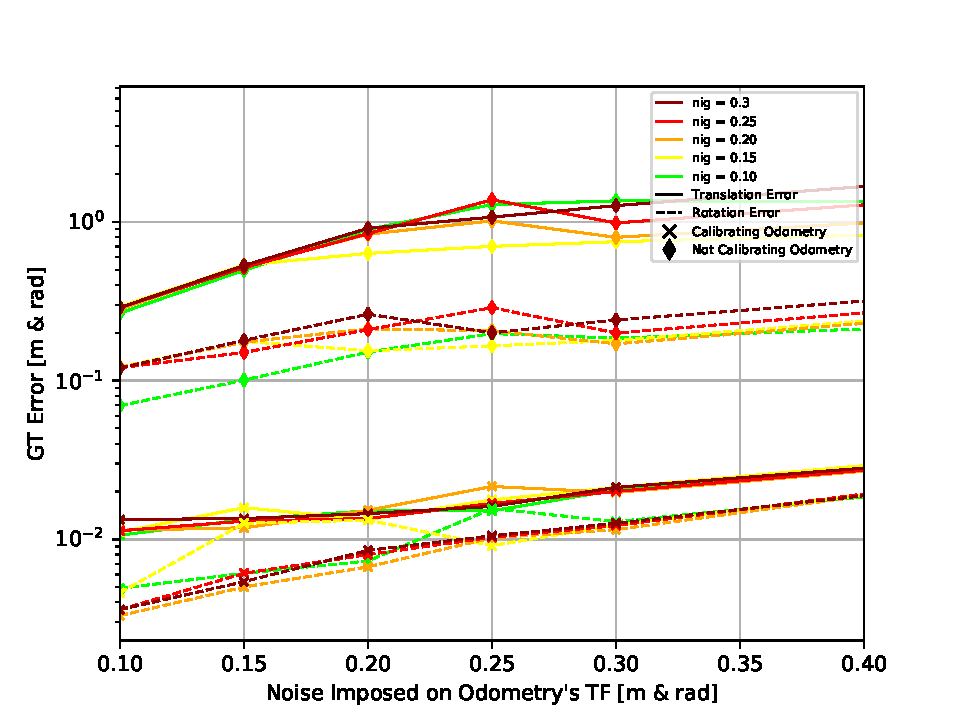
\includegraphics[width=0.5\textwidth]{resources/Translation_&_Rotation_error_compared_to_GT_caused_by_imposing_noise_on_the_odometry_calibrating_odometry_OVERLAPPED.pdf} \\
      \caption{\label{fig:trGTntfvCalib}Translation and Rotation error compared to ground truth caused by imposing noise on the
      geometrical transformation of the odometry for different values of noise imposed on the geometrical
    transformations of the sensors, \textbf{calibrating the transformation provided by the  odometry}}
    \end{figure}

\section{Conclusion}

This dissertation proposed a methodology to extrinsically calibrate robotic vehicles with inaccurate odometry data, building on top of
\textit{atom} a multi-modal and multi-sensor calibration framework. This framework approaches calibration as an
extended optimization problem, in which the poses of the sensors along with the poses of the pattern are also
estimated. By carefully modifying the input parameters of the optimizer to include additionally the
transformations provided by the odometry systems, these could also be estimated, allowing \textit{atom} to
calibrate robotic vehicles with inaccurate odometry data. To test the proposed methodology in a controlled simulated environment,
an algorithm to recreate realistic noise on the \textit{tf} of the robotic systems was developed. The methodology
proved to be successful, enabling \textit{softbot}, a simulated robot designed for calibrating sensors \textit{wrt}
to the motion coordinate frame of the robot, to achieve calibration errors that were an entire order of
magnitude lower than those observed in an exact robot configuration without the proposed approach, across a
wide range of imposed noise levels both to the transformations of the sensors being calibrated, and the one
provided by the odometry system. 

Transposing the methodology from simulation to \textit{ZAU}, a real robot, posed several challenges that
ultimately led to the inability to calibrate the system. Given that \textit{ZAU} exhibited odometry errors
uncharacteristic of an advanced odometry system, further testing would have been needed to determine whether the issue
lies in a faulty odometry system or a limitation of the methodology.

Future work should start by testing the methodology with other real robots to expand the understanding of
its limitations. One of the main shortcomings of this approach is that one would have to use
the data from a single odometry source even if more were available, such as in \textit{ZAU}. After evaluating
the limitations of the methodology, the subsequent step in this research should be to integrate multiple odometry
sources. Kalman filters, which are widely used for fusing data from multiple sensors, could be the key to
advancing this research. Other import research direction would be to integrate other methodologies that
calibrate the kinematic parameters of the odometry system to see if the use of both methodologies
simultaneously improve the calibration results.

\EOD
\end{document}
